% Provenance (never printed): lycee terminale S SVT "Les climats de la Terre"
% and the 2019 enseignement scientifique ("Le climat de la Terre": forcing,
% feedbacks, the IPCC assessments, scenarios), union; physical science only,
% as the user ruled (2026-10-22). See sources/outline_sources.md. Pilot
% chapter, 2026-10-22. Every figure about the climate system is an IPCC AR6
% WG1 statement (ledger ipcc:*) or computed from a dataset in
% figdata/grade-12/climate_records.py.
\chapter{Climate Change: Observations, Causes and Projections}\label{ch:g12:climate-change}

High on the northern slope of Mauna Loa, a volcano in the middle of the
Pacific Ocean, a cluster of white buildings stands on bare lava,
\qty{3397}{m} above the sea. Up there, above the layer of air polluted by
the island below and thousands of kilometres from any large city, the air
is about as clean and well mixed as the atmosphere of the whole planet. Since
March 1958, its carbon dioxide has been measured almost without a break.
The record began as one chemist's project; it has become the most famous
curve in Earth science. This chapter reads that curve and the other records
of the climate, explains how a change in the air changes the \omterm{def:g10:earth-energy-budget:energy-budget}{energy budget}
of the planet, how scientists decide what caused the warming they observe,
and what they project for the decades to come.
% ledger: noaa:mlo-site, noaa:keeling-1958

\begin{omfigure}
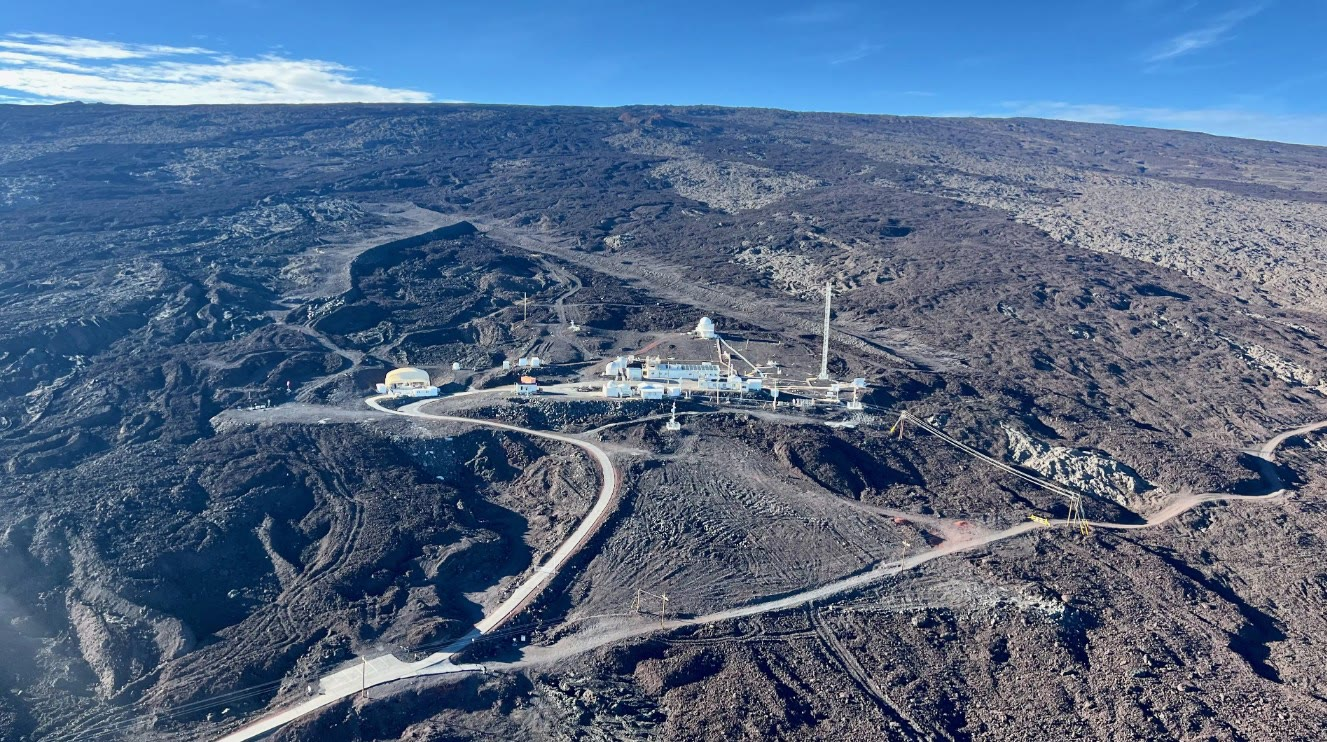
\includegraphics[width=0.78\linewidth]{images/book2/g12-noaa-mauna-loa-observatory.jpg}

{\small The Mauna Loa Observatory, Hawaii, on old lava flows high on the
north flank of the volcano. Photograph: Brian Vasel, NOAA (public domain).}
\end{omfigure}

\begin{recall}
The Earth receives energy from the Sun as light and loses the same amount on
average to space as infrared radiation; the fraction of sunlight reflected
is the \omterm{def:g10:earth-energy-budget:albedo}{albedo} (\cref{ch:g10:earth-energy-budget}). Greenhouse gases --- water
vapour, carbon dioxide, methane --- absorb part of the infrared that the
surface emits and send part of it back down; this greenhouse effect keeps
the surface far warmer than it would otherwise be (the chemistry books, and
Book 1, grade 9). \omterm{def:g12:past-climates:ice-core}{Ice cores} keep bubbles of ancient air and record the
\omterm{def:g12:past-climates:glacial-cycle}{glacial cycles} of the last 800\,000 years (\cref{ch:g12:past-climates}).
\end{recall}

\section{The records}

\begin{omfigure}
\begin{tikzpicture}
\begin{axis}[omrecord, width=0.92\linewidth, height=6.2cm, xmin=1957, xmax=2028,
  ymin=305, ymax=440, xlabel={year}, ylabel={carbon dioxide (ppm)},
  xtick={1960,1970,...,2020}, /pgf/number format/1000 sep={}]
\addplot[omDef!85!black, line width=0.5pt] table[x=decimal_year, y=co2_ppm] {figdata/out/grade-12-climate_records-co2.dat};
\addplot[only marks, mark=*, mark size=0.9pt, omThm!85!black] table[x=year, y=co2_ppm] {figdata/out/grade-12-climate_records-co2annual.dat};
\end{axis}
\end{tikzpicture}

{\small The carbon dioxide content of the air at Mauna Loa: monthly means
(line) and annual means (dots), in parts per million (ppm) of dry air.
Data: NOAA Global Monitoring Laboratory and Scripps Institution of
Oceanography.}
\end{omfigure}

\begin{proposition}[The carbon dioxide record]\label{prop:g12:climate-change:co2}
% ledger: data:co2-mlo (all numbers computed in figdata/grade-12/climate_records.py)
At Mauna Loa, the annual mean concentration of carbon dioxide rose from
\qty{316.0}{ppm} in 1959 to \qty{427.4}{ppm} in 2025, and the rise is
getting faster: the concentration grew by about \qty{0.9}{ppm} per year in
the 1960s and by about \qty{2.6}{ppm} per year between 2015 and 2025. Every
year the concentration also swings by about \qty{7}{ppm}: it is highest in
May and lowest in September.
\end{proposition}

\begin{remark}[Why the curve has teeth]\label{rem:g12:climate-change:teeth}
The yearly swing is the breathing of the vegetation of the Northern
Hemisphere, where most land plants are. In spring and summer, plants take
up more carbon dioxide by photosynthesis than they and the soil release;
in autumn and winter, decay and respiration win. The rise from year to
year is a different story: it is the carbon of fossil fuels and of cleared
forests accumulating in the air.
\end{remark}

\begin{proposition}[Higher than for at least two million years]\label{prop:g12:climate-change:icecore}
% ledger: data:co2-bereiter (173.7 and 298.6 ppm computed), ipcc:co2-2myr (high confidence)
Over the last 800\,000 years, the air bubbles of Antarctic ice record
carbon dioxide concentrations between about \qty{174}{ppm}, in the coldest
\omterm{def:g12:past-climates:glacial-cycle}{glacial periods}, and \qty{299}{ppm}, in the warmest \omterm{def:g12:past-climates:glacial-cycle}{interglacials}. Today's
value lies more than \qty{100}{ppm} above the highest of them. The
assessments state that the concentration in 2019 was higher than at any time
in at least two million years (\emph{high confidence}).
\end{proposition}

\begin{omfigure}
\begin{tikzpicture}
\begin{axis}[omrecord, omage, width=0.92\linewidth, height=5.2cm, xmin=0, xmax=810,
  ymin=150, ymax=490, xlabel={thousands of years before 1950},
  ylabel={carbon dioxide (ppm)}, xtick={0,100,...,800}]
\addplot[omDef!85!black, line width=0.6pt] table[x=age_kyr, y=co2_ppm] {figdata/out/grade-12-climate_records-icecore.dat};
\draw[omThm, densely dashed, line width=0.8pt] (axis cs:810,427.35) -- (axis cs:0,427.35);
\node[font=\footnotesize, text=omThm!85!black, anchor=south west] at (axis cs:780,433) {annual mean at Mauna Loa in 2025};
\end{axis}
\end{tikzpicture}

{\small Carbon dioxide in Antarctic ice over 800\,000 years: the \omterm{def:g12:past-climates:glacial-cycle}{glacial
cycles} move it between about 180 and \qty{300}{ppm}. The thin spike at the
right-hand end is the youngest ice, which records the start of the present
rise, up to the year 2001. Data: Bereiter and others (2015), NOAA
Paleoclimatology.}
% the youngest sample of the composite: age -51 yr BP (2001), 368.02 ppm (data/derived/co2-icecore.csv)
\end{omfigure}

\begin{omfigure}
\begin{tikzpicture}
\begin{axis}[omrecord, width=0.92\linewidth, height=5.6cm, xmin=1878, xmax=2027,
  ymin=-0.6, ymax=1.45, xlabel={year},
  ylabel={temperature anomaly (\unit{\degreeCelsius})},
  xtick={1880,1900,...,2020}, /pgf/number format/1000 sep={},
  legend style={at={(0.03,0.96)}, anchor=north west, font=\footnotesize, draw=black!30}]
\addplot[omDef!70, line width=0.5pt, mark=*, mark size=0.6pt] table[x=year, y=anomaly] {figdata/out/grade-12-climate_records-temp.dat};
\addlegendentry{annual mean}
\addplot[omThm!85!black, line width=1.3pt, unbounded coords=jump] table[x=year, y=mean11] {figdata/out/grade-12-climate_records-temp.dat};
\addlegendentry{11-year average}
\end{axis}
\end{tikzpicture}

{\small Global mean surface temperature, as the difference from its average
over 1951--1980. Data: NASA GISS Surface Temperature Analysis (GISTEMP v4).}
\end{omfigure}

\begin{proposition}[Global warming observed]\label{prop:g12:climate-change:warming}
% ledger: ipcc:gsat-2011-2020, ipcc:decades
Each of the last four decades has been warmer than any decade before it
since 1850. The global surface temperature of 2011--2020 was \qty{1.09}{\degreeCelsius}
higher than that of 1850--1900 (very likely between 0.95 and
\qty{1.20}{\degreeCelsius}), with more warming over land
(\qty{1.59}{\degreeCelsius}) than over the ocean (\qty{0.88}{\degreeCelsius}).
\end{proposition}

\begin{proposition}[Sea level rises faster and faster]\label{prop:g12:climate-change:sea}
% ledger: ipcc:sea-level-obs, data:gmsl-lsa (3.2 mm/yr trend computed)
Global mean sea level rose by about \qty{0.20}{m} between 1901 and 2018.
The rate was about \qty{1.3}{mm} per year from 1901 to 1971,
\qty{1.9}{mm} per year from 1971 to 2006 and \qty{3.7}{mm} per year from
2006 to 2018 (\emph{high confidence}). Satellites, measuring the height of
the sea surface since 1993, find an average of \qty{3.2}{mm} per year over
1993--2025. The sea rises because the warming ocean expands and because
glaciers and ice sheets lose ice to it.
\end{proposition}

\begin{omfigure}
\begin{tikzpicture}
\begin{axis}[omrecord, width=0.86\linewidth, height=5cm, xmin=1992, xmax=2026,
  ymin=-35, ymax=95, xlabel={year}, ylabel={sea level (mm)},
  /pgf/number format/1000 sep={}, xtick={1995,2000,...,2025}]
\addplot[omDef!85!black, line width=0.5pt] table[x=decimal_year, y=gmsl_mm] {figdata/out/grade-12-climate_records-sea.dat};
\end{axis}
\end{tikzpicture}

{\small Global mean sea level measured from space, about every ten days
(seasonal signal removed), relative to an arbitrary zero. Altimetry data are
provided by NOAA Laboratory for Satellite Altimetry.}
\end{omfigure}

\begin{dated}{2025}
% ledger: data:co2-mlo, data:gistemp (values read from the datasets as fetched 2026-10-22)
The annual mean carbon dioxide concentration at Mauna Loa in 2025 was
\qty{427.35}{ppm}. In the NASA temperature record, the warmest year so far
was 2024, at \qty{1.28}{\degreeCelsius} above the 1951--1980 average.
\end{dated}

\section{Radiative forcing}

\begin{definition}[Radiative forcing]\label{def:g12:climate-change:forcing}
The \emph{radiative forcing}\index{radiative forcing} of a change in the
climate system --- more greenhouse gas, more aerosol particles, a brighter
Sun --- is the change it causes in the net flow of energy entering the
climate system at the top of the atmosphere, before the surface temperature
has had time to respond. It is measured in watts per square metre
(\unit{W/m^2}) of the Earth's surface. A positive forcing makes the planet
gain energy and warm; a negative forcing makes it lose energy and cool.
\end{definition}

\begin{remark}[Effective forcing]\label{rem:g12:climate-change:effective}
The assessments use the \emph{effective} \omterm{def:g12:climate-change:forcing}{radiative forcing}, which also
counts the fast adjustments of the atmosphere (of its clouds, for instance)
that happen before the surface warms. All the \omterm{def:g12:climate-change:forcing}{forcings} of this chapter are
effective \omterm{def:g12:climate-change:forcing}{forcings}.
\end{remark}

\begin{proposition}[The forcing since 1750]\label{prop:g12:climate-change:forcing}
% ledger: ipcc:erf-total, ipcc:erf-agents
Human activities have produced a total \omterm{def:g12:climate-change:forcing}{radiative forcing} of
\qty{2.72}{W/m^2} in 2019 relative to 1750 (very likely between 1.96 and
\qty{3.48}{W/m^2}). The greenhouse gases contribute a positive \omterm{def:g12:climate-change:forcing}{forcing}, led
by carbon dioxide (\qty{2.16}{W/m^2}); aerosol particles, which reflect
sunlight and brighten clouds, contribute a negative one (about
\qty{-1.06}{W/m^2} in all). The change in the Sun's brightness over the
same period contributes only \qty{0.01}{W/m^2}.
\end{proposition}

\begin{omfigure}
% ledger: ipcc:erf-agents, ipcc:erf-total (central values and 5-95 % ranges of AR6 Table 7.8)
\begin{tikzpicture}
\begin{axis}[xbar, width=0.8\linewidth, height=7.2cm, xmin=-1.8, xmax=3.7,
  ytick={1,...,10}, yticklabels={total (human), solar, land use,
  aerosol--cloud, aerosol--radiation, ozone, halogenated gases, nitrous oxide,
  methane, carbon dioxide}, y tick label style={font=\small},
  tick label style={font=\small}, xlabel={effective radiative forcing, 1750--2019 (\unit{W/m^2})},
  label style={font=\small}, bar width=6pt, bar shift=0pt, axis x line=bottom, axis y line=left,
  axis line style={-}, enlarge y limits=0.07, xmajorgrids,
  grid style={gray!22, line width=0.3pt}, extra x ticks={0},
  extra x tick style={grid style={black!60, line width=0.5pt}}]
\addplot[fill=omThm!55, draw=omThm!80!black, error bars/.cd, x dir=both, x explicit,
  error bar style={black!70}] coordinates {
  (2.16,10) += (0.25,0) -= (0.26,0)
  (0.54,9) += (0.11,0) -= (0.11,0)
  (0.21,8) += (0.03,0) -= (0.03,0)
  (0.41,7) += (0.08,0) -= (0.08,0)
  (0.47,6) += (0.24,0) -= (0.23,0)
  (2.72,1) += (0.76,0) -= (0.76,0)
  (0.01,2) += (0.07,0) -= (0.07,0)};
\addplot[fill=omDef!55, draw=omDef!80!black, error bars/.cd, x dir=both, x explicit,
  error bar style={black!70}] coordinates {
  (-0.22,5) += (0.26,0) -= (0.25,0)
  (-0.84,4) += (0.59,0) -= (0.61,0)
  (-0.20,3) += (0.10,0) -= (0.10,0)};
\end{axis}
\end{tikzpicture}

{\small The main effective \omterm{def:g12:climate-change:forcing}{radiative forcings} from 1750 to 2019, with their
very likely ranges (whiskers). Values: IPCC Sixth Assessment Report, Working
Group~I, Table 7.8.}
\end{omfigure}

\begin{proposition}[Carbon dioxide: each doubling adds the same forcing]\label{prop:g12:climate-change:log}
% ledger: ipcc:erf-2xco2, ipcc:log-co2
To a good approximation, the \omterm{def:g12:climate-change:forcing}{forcing} of carbon dioxide grows with the
\emph{logarithm} of its concentration: each doubling adds the same \omterm{def:g12:climate-change:forcing}{forcing},
$F_{2\times} = \qty{3.93}{W/m^2}$ for a doubling from the concentration of
1750, $C_0 = \qty{278}{ppm}$. The \omterm{def:g12:climate-change:forcing}{forcing} of a concentration $C$ is then
\[
  F = F_{2\times}\,\frac{\ln (C/C_0)}{\ln 2}.
\]
\end{proposition}

\begin{example}[Checking the law against the assessment]\label{ex:g12:climate-change:check}
% ledger: ipcc:erf-2xco2, ipcc:erf-agents
In 2019 the concentration was \qty{410}{ppm}. The law gives
$F = 3.93 \times \ln(410/278)/\ln 2 = 3.93 \times 0.561 \approx
\qty{2.20}{W/m^2}$, within 2\,\% of the \qty{2.16}{W/m^2} that the
assessment gives for carbon dioxide over 1750--2019.
\end{example}

\begin{proposition}[Where the extra energy goes]\label{prop:g12:climate-change:heating}
% ledger: ipcc:heating
Because the \omterm{def:g12:climate-change:forcing}{forcing} is positive, the climate system gains energy: about
\qty{0.79}{W/m^2} on average over 2006--2018, up from \qty{0.50}{W/m^2} over
1971--2006 (\emph{high confidence}). The ocean took 91\,\% of this energy; the
land 5\,\%, the melting ice 3\,\% and the atmosphere only 1\,\%.
\end{proposition}

\section{Feedbacks and climate sensitivity}

When the surface warms, it radiates more energy to space, which tends to
bring the planet back into balance. But the warming also changes other
things --- the water vapour in the air, the snow and ice on the ground, the
clouds --- and these changes alter the \omterm{def:g10:earth-energy-budget:energy-budget}{energy budget} in their turn.

\begin{definition}[Climate feedback]\label{def:g12:climate-change:feedback}
A \emph{climate feedback}\index{climate feedback} is a change in the climate
system, caused by a change in temperature, that alters the \omterm{def:g10:earth-energy-budget:energy-budget}{energy budget}
and so the temperature change itself. A \emph{positive feedback} amplifies
the initial change; a \emph{negative feedback} damps it.
\end{definition}

\begin{example}[Three feedbacks]\label{ex:g12:climate-change:three}
\begin{itemize}
  \item \textbf{Water vapour (positive).} Warmer air holds more water
        vapour, a greenhouse gas, which adds to the warming.
  \item \textbf{Snow and ice (positive).} Snow and ice reflect sunlight;
        when they melt, the darker land and sea beneath absorb more of it,
        and the warming grows.
  \item \textbf{Radiation to space (negative).} A warmer surface and
        atmosphere radiate more infrared to space. This basic response
        always wins in the end: it is why the climate settles at a new,
        warmer balance instead of warming without limit.
\end{itemize}
\end{example}

\begin{omfigure}
\begin{tikzpicture}[font=\small, >={Stealth[length=2.4mm]},
  box/.style={draw=black!60, rounded corners=2pt, fill=white, align=center,
  inner sep=3pt, text width=3cm}]
  \node[box, fill=omThm!12] (w) at (0,0) {surface warms};
  \node[box] (v) at (3.6,1.3) {more water vapour in the air};
  \node[box] (g) at (3.6,-1.3) {stronger\\greenhouse effect};
  \draw[->, omThm!85!black, thick] (w) to[bend left=18] (v);
  \draw[->, omThm!85!black, thick] (v) -- (g);
  \draw[->, omThm!85!black, thick] (g) to[bend left=18] (w);
  \node[font=\footnotesize, text=omThm!85!black] at (2.0,0) {$+$};
  \node[box] (s) at (-3.6,1.3) {snow and ice melt};
  \node[box] (a) at (-3.6,-1.3) {lower albedo: more sunlight absorbed};
  \draw[->, omThm!85!black, thick] (w) to[bend right=18] (s);
  \draw[->, omThm!85!black, thick] (s) -- (a);
  \draw[->, omThm!85!black, thick] (a) to[bend right=18] (w);
  \node[font=\footnotesize, text=omThm!85!black] at (-2.0,0) {$+$};
  \node[box] (r) at (0,-2.9) {more infrared radiated to space};
  \draw[->, omDef!85!black, thick] ([xshift=-0.35cm]w.south) -- ([xshift=-0.35cm]r.north);
  \draw[->, omDef!85!black, thick] ([xshift=0.35cm]r.north) -- ([xshift=0.35cm]w.south);
  \node[font=\footnotesize, text=omDef!85!black] at (0.62,-1.45) {$-$};
\end{tikzpicture}

{\small Two positive \omterm{def:g12:climate-change:feedback}{feedbacks} (red loops) amplify a warming; the extra
infrared radiated by a warmer planet (blue) is a negative \omterm{def:g12:climate-change:feedback}{feedback} that
limits it.}
\end{omfigure}

\begin{proposition}[Warming at equilibrium]\label{prop:g12:climate-change:equilibrium}
% ledger: ipcc:feedbacks
Once the climate has reached a new balance, the warming $\Delta T$ caused by
a constant \omterm{def:g12:climate-change:forcing}{forcing} $F$ is
\[
  \Delta T = \frac{F}{\lambda},
\]
where $\lambda$, the \emph{\omterm{def:g12:climate-change:feedback}{climate feedback} parameter}, is the extra energy
the planet loses to space for each degree of warming. The assessments
combine the radiation to space ($\qty{3.22}{W.m^{-2}.\degreeCelsius^{-1}}$)
with the positive \omterm{def:g12:climate-change:feedback}{feedbacks} of water vapour and the temperature profile
($1.30$), of surface \omterm{def:g10:earth-energy-budget:albedo}{albedo} ($0.35$) and of clouds ($0.42$, in the same
unit) into $\lambda \approx \qty{1.16}{W.m^{-2}.\degreeCelsius^{-1}}$.
\end{proposition}

\begin{proof}[Partial proof]
At the new balance the climate system again loses to space as much energy
as it gains, so the extra loss due to the warming, $\lambda\,\Delta T$, must
make up for the \omterm{def:g12:climate-change:forcing}{forcing}: $\lambda\,\Delta T = F$. That the extra loss is
proportional to $\Delta T$ is an approximation, good for warmings of a few
degrees, and admitted here.
\end{proof}

\begin{definition}[Equilibrium climate sensitivity]\label{def:g12:climate-change:ecs}
The \emph{equilibrium climate sensitivity}\index{equilibrium climate sensitivity}
is the warming of the Earth's surface, once a new balance is reached, after
the concentration of carbon dioxide has been doubled from its 1750 level.
\end{definition}

\begin{proposition}[How sensitive is the climate?]\label{prop:g12:climate-change:ecs}
% ledger: ipcc:ecs
Combining all the lines of evidence --- the physics of the \omterm{def:g12:climate-change:feedback}{feedbacks}, the
observed warming, past climates --- the assessments give a best estimate
of \qty{3}{\degreeCelsius} for the \omterm{def:g12:climate-change:ecs}{equilibrium climate sensitivity}, likely
between 2.5 and \qty{4}{\degreeCelsius} (\emph{high confidence}), and very
likely between 2 and \qty{5}{\degreeCelsius}.
\end{proposition}

\section{Who is responsible?}

\begin{method}[Reading a statement of the assessments]\label{met:g12:climate-change:language}
% ledger: ipcc:likelihood
The international assessments of climate science grade every finding in a
fixed vocabulary, printed in italics:
\begin{itemize}
  \item a \emph{likelihood}, the probability of an outcome:
        \emph{virtually certain} 99--100\,\%, \emph{extremely likely}
        95--100\,\%, \emph{very likely} 90--100\,\%, \emph{likely}
        66--100\,\%, \emph{about as likely as not} 33--66\,\%,
        \emph{unlikely} 0--33\,\%, \emph{very unlikely} 0--10\,\%;
  \item a \emph{confidence}, the strength of the evidence and the agreement
        behind a finding: very low, low, medium, high, very high.
\end{itemize}
A range written $[x \text{ to } y]$ is a very likely range: there is a 90\,\%
chance that the true value lies inside it. To read a statement, identify
the quantity, its best estimate, its range, and the likelihood or
confidence attached.
\end{method}

\begin{definition}[Attribution]\label{def:g12:climate-change:attribution}
\emph{Attribution}\index{attribution} is the assessment of how much of an
observed change is due to each of its possible causes, with the likelihood
of the result.
\end{definition}

\begin{proposition}[Human influence]\label{prop:g12:climate-change:attribution}
% ledger: ipcc:unequivocal, ipcc:attribution, ipcc:observed-2010-2019
It is unequivocal that human influence has warmed the atmosphere, the ocean
and the land. Between 1850--1900 and 2010--2019, the global surface warmed by
about \qty{1.06}{\degreeCelsius}. Human activities caused a warming of
\qty{0.8}{\degreeCelsius} to \qty{1.3}{\degreeCelsius} (likely range), best
estimate \qty{1.07}{\degreeCelsius}: the well-mixed greenhouse gases likely
warmed the surface by 1.0 to \qty{2.0}{\degreeCelsius}, and the other human
influences, mainly aerosols, likely cooled it by 0 to
\qty{0.8}{\degreeCelsius}. The Sun and volcanoes changed it by only $-0.1$
to $+\qty{0.1}{\degreeCelsius}$, and the natural fluctuations of the climate
by $-0.2$ to $+\qty{0.2}{\degreeCelsius}$.
\end{proposition}

\begin{omfigure}
% ledger: ipcc:attribution, ipcc:observed-2010-2019
\begin{tikzpicture}
\begin{axis}[width=0.7\linewidth, height=5.6cm, xmin=-1, xmax=2.2, ymin=0.4, ymax=6.6,
  ytick={1,...,6}, yticklabels={natural variability, Sun and volcanoes,
  aerosols and other human, greenhouse gases, all human influences, observed},
  y tick label style={font=\small}, tick label style={font=\small},
  xlabel={contribution to the warming 1850--1900 to 2010--2019 (\unit{\degreeCelsius})},
  label style={font=\small}, axis x line=bottom, axis y line=left, axis line style={-},
  xmajorgrids, grid style={gray!22, line width=0.3pt}, extra x ticks={0},
  extra x tick style={grid style={black!60, line width=0.5pt}}]
\draw[black!70, line width=5pt] (axis cs:0.88,6) -- (axis cs:1.21,6);
\fill (axis cs:1.06,6) circle (2.4pt);
\draw[omThm!80, line width=5pt] (axis cs:0.8,5) -- (axis cs:1.3,5);
\fill (axis cs:1.07,5) circle (2.4pt);
\draw[omThm!55, line width=5pt] (axis cs:1.0,4) -- (axis cs:2.0,4);
\draw[omDef!60, line width=5pt] (axis cs:-0.8,3) -- (axis cs:0,3);
\draw[gray!70, line width=5pt] (axis cs:-0.1,2) -- (axis cs:0.1,2);
\draw[gray!45, line width=5pt] (axis cs:-0.2,1) -- (axis cs:0.2,1);
\end{axis}
\end{tikzpicture}

{\small What caused the observed warming: likely ranges of each contribution,
with the best estimates where the assessment gives one (dots); for the
observed warming, its very likely range. Values: IPCC Sixth Assessment
Report, Working Group~I, Summary for Policymakers, A.1.3.}
\end{omfigure}

\section{Scenarios and projections}

\begin{definition}[Scenario and projection]\label{def:g12:climate-change:scenario}
An \emph{emission scenario}\index{emission scenario} is a consistent
story of how the emissions of greenhouse gases and aerosols might evolve in
the future. A \emph{projection}\index{projection (climate)} is the response
of the climate computed by models for a given scenario. A projection is not
a forecast: it says what would happen \emph{if} the scenario came true.
\end{definition}

\begin{proposition}[Projected warming and sea-level rise]\label{prop:g12:climate-change:projections}
% ledger: ipcc:proj-temp, ipcc:proj-sea, ipcc:3myr
The assessments use five main \omterm{def:g12:climate-change:scenario}{scenarios}, from very low emissions (SSP1-1.9)
to very high emissions (SSP5-8.5). For 2081--2100, compared with 1850--1900,
they project the warmings below (best estimates and very likely ranges, in
\unit{\degreeCelsius}), and, by 2100, the likely rises of global mean sea
level relative to 1995--2014. Under every \omterm{def:g12:climate-change:scenario}{scenario} the sea keeps rising
through the century (\emph{virtually certain}). The last time the global
surface stayed \qty{2.5}{\degreeCelsius} or more above 1850--1900 was over
three million years ago (\emph{medium confidence}).

\begin{center}
\small
\begin{tabular}{lccc}
\hline
\omterm{def:g12:climate-change:scenario}{scenario} & emissions & warming 2081--2100 (\unit{\degreeCelsius}) & sea-level rise by 2100 (m) \\
\hline
SSP1-1.9 & very low & 1.4 (1.0 to 1.8) & 0.28 to 0.55 \\
SSP1-2.6 & low & 1.8 (1.3 to 2.4) & 0.32 to 0.62 \\
SSP2-4.5 & intermediate & 2.7 (2.1 to 3.5) & 0.44 to 0.76 \\
SSP3-7.0 & high & 3.6 (2.8 to 4.6) & --- \\
SSP5-8.5 & very high & 4.4 (3.3 to 5.7) & 0.63 to 1.01 \\
\hline
\end{tabular}
\end{center}
\end{proposition}

\begin{omfigure}
% ledger: ipcc:proj-temp
\begin{tikzpicture}
\begin{axis}[width=0.8\linewidth, height=5.2cm, xmin=0.4, xmax=5.6, ymin=0, ymax=6.2,
  xtick={1,...,5}, xticklabels={SSP1-1.9, SSP1-2.6, SSP2-4.5, SSP3-7.0, SSP5-8.5},
  x tick label style={font=\small}, tick label style={font=\small},
  ylabel={warming 2081--2100 (\unit{\degreeCelsius})}, label style={font=\small},
  axis x line=bottom, axis y line=left, axis line style={-}, ymajorgrids,
  grid style={gray!22, line width=0.3pt}]
\draw[omThm!60, line width=9pt] (axis cs:1,1.0) -- (axis cs:1,1.8);
\draw[black, line width=1.2pt] (axis cs:0.83,1.4) -- (axis cs:1.17,1.4);
\draw[omThm!60, line width=9pt] (axis cs:2,1.3) -- (axis cs:2,2.4);
\draw[black, line width=1.2pt] (axis cs:1.83,1.8) -- (axis cs:2.17,1.8);
\draw[omThm!60, line width=9pt] (axis cs:3,2.1) -- (axis cs:3,3.5);
\draw[black, line width=1.2pt] (axis cs:2.83,2.7) -- (axis cs:3.17,2.7);
\draw[omThm!60, line width=9pt] (axis cs:4,2.8) -- (axis cs:4,4.6);
\draw[black, line width=1.2pt] (axis cs:3.83,3.6) -- (axis cs:4.17,3.6);
\draw[omThm!60, line width=9pt] (axis cs:5,3.3) -- (axis cs:5,5.7);
\draw[black, line width=1.2pt] (axis cs:4.83,4.4) -- (axis cs:5.17,4.4);
\end{axis}
\end{tikzpicture}

{\small Projected warming at the end of the century for the five \omterm{def:g12:climate-change:scenario}{scenarios}:
very likely range (bar) and best estimate (black line). Values: IPCC Sixth
Assessment Report, Working Group~I, Table SPM.1.}
\end{omfigure}

\begin{remark}[What this chapter does not say]\label{rem:g12:climate-change:science}
Which \omterm{def:g12:climate-change:scenario}{scenario} the world will follow depends on future emissions, that is,
on decisions that are not questions of physics. The physical science says
how the climate responds to each one; the choice among them belongs to
societies, and its costs and benefits are studied by other sciences.
\end{remark}

\begin{history}[A curve that started as a chemist's project]
% ledger: noaa:keeling-1958
In March 1958 the chemist Charles David Keeling, of the Scripps Institution
of Oceanography, began measuring the carbon dioxide of the air at Mauna Loa
with an instrument precise enough to see changes of a fraction of a part
per million. Within a few years his record showed both the yearly breathing
of the vegetation and a steady rise. The measurements, continued since by
Scripps and by the US weather and ocean agency, are the longest direct record
of the composition of the atmosphere.
\begin{center}
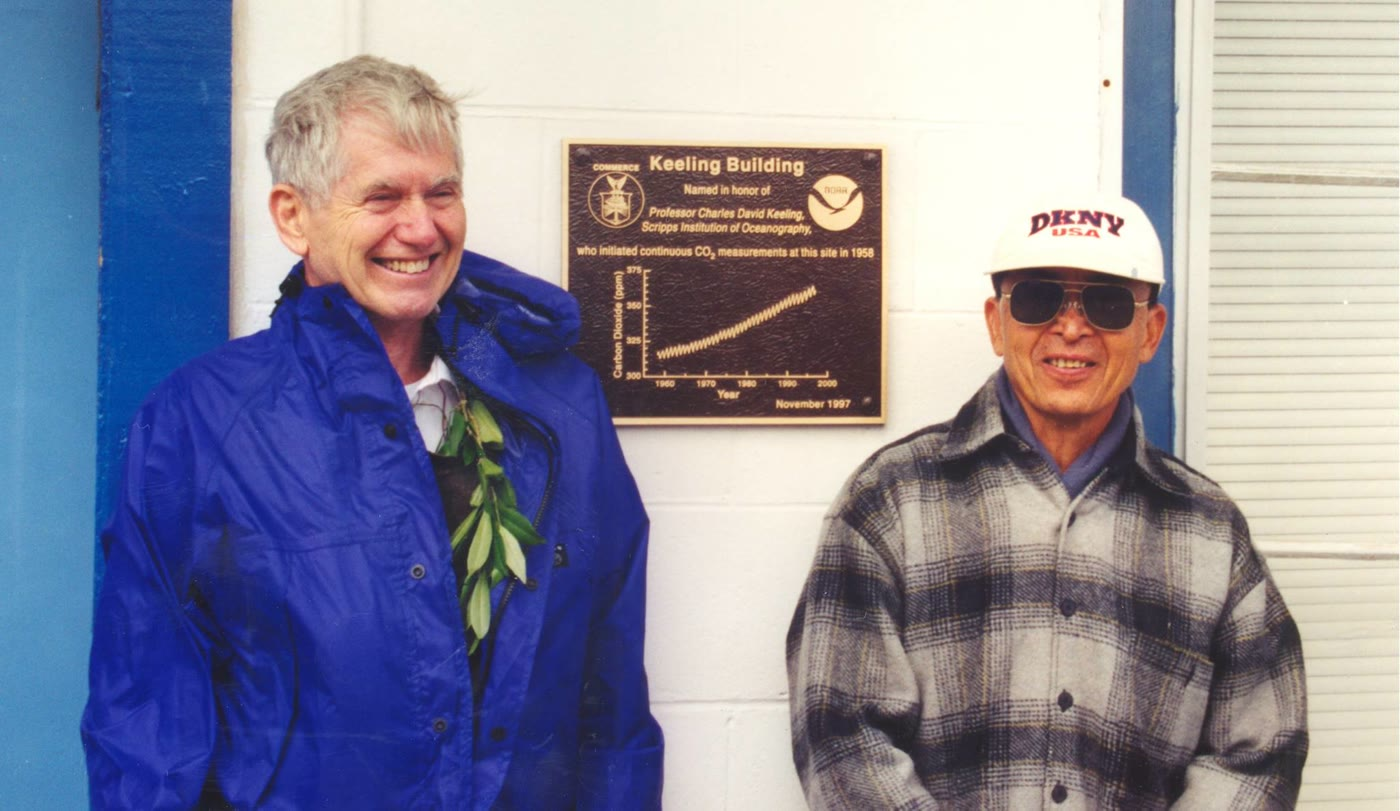
\includegraphics[width=0.62\linewidth]{images/book2/g12-noaa-keeling-chin-1997.jpg}

{\small Charles David Keeling (left) and John Chin at the Mauna Loa
Observatory in 1997, beside the plaque that names a building after Keeling.
Photograph: John Miller, NOAA (public domain).}
\end{center}
\end{history}

\section{Exercises}

\begin{exercise}[$\star$]\label{exo:g12:climate-change:1}
What is the \omterm{def:g12:climate-change:forcing}{radiative forcing} of a change in the climate system? In which
unit is it measured, and what does its sign mean?
\end{exercise}

\begin{exercise}[$\star$]\label{exo:g12:climate-change:2}
In which month of the year is the carbon dioxide concentration at Mauna Loa
highest, and in which is it lowest? Explain the yearly swing.
\end{exercise}

\begin{exercise}[$\star$]\label{exo:g12:climate-change:3}
In the vocabulary of the assessments, what probability does \emph{very
likely} mean? And \emph{likely}? What does a range written
$[0.95 \text{ to } 1.20]$ mean?
\end{exercise}

\begin{exercise}[$\star$]\label{exo:g12:climate-change:4}
Of the extra energy that the climate system has gained in recent decades,
what share went into the ocean? Why does this explain why sea level rises
even without melting ice?
\end{exercise}

\begin{exercise}[$\star$]\label{exo:g12:climate-change:5}
Give two positive \omterm{def:g12:climate-change:feedback}{climate feedbacks} and the negative response that limits
the warming. Explain each in one sentence.
\end{exercise}

\begin{exercise}[$\star\star$]\label{exo:g12:climate-change:6}
The annual mean concentration of carbon dioxide at Mauna Loa was
\qty{315.98}{ppm} in 1959 and \qty{427.35}{ppm} in 2025. By how many ppm,
and by what percentage, did it increase? What was the average growth per
year over the whole period?
\end{exercise}

\begin{exercise}[$\star\star$]\label{exo:g12:climate-change:7}
Use the logarithmic law of the chapter, with $F_{2\times} =
\qty{3.93}{W/m^2}$ and $C_0 = \qty{278}{ppm}$, to compute the \omterm{def:g12:climate-change:forcing}{forcing} of
carbon dioxide at \qty{427.35}{ppm}, the 2025 annual mean.
\end{exercise}

\begin{exercise}[$\star\star$]\label{exo:g12:climate-change:8}
At \qty{3.7}{mm} per year, the rate of 2006--2018, how much would sea level
rise in 30 years? How many times faster is this rate than that of
1901--1971, \qty{1.3}{mm} per year?
\end{exercise}

\begin{exercise}[$\star\star$]\label{exo:g12:climate-change:9}
Using $\Delta T = F/\lambda$ with $\lambda = \qty{1.16}{W.m^{-2}.\degreeCelsius^{-1}}$,
compute the equilibrium warming that the total human \omterm{def:g12:climate-change:forcing}{forcing} of 2019,
\qty{2.72}{W/m^2}, would produce. The observed human-caused warming is only
about \qty{1.07}{\degreeCelsius}. Give the main reason for the difference.
\end{exercise}

\begin{exercise}[$\star\star$]\label{exo:g12:climate-change:10}
The Sun and volcanoes changed the global temperature between 1850--1900 and
2010--2019 by $-0.1$ to $+\qty{0.1}{\degreeCelsius}$, while the observed
warming was about \qty{1.06}{\degreeCelsius}. What can you conclude? Which
other natural cause must also be ruled out, and what does the assessment
say about it?
\end{exercise}

\begin{exercise}[$\star\star$]\label{exo:g12:climate-change:11}
Using the table of \omterm{def:g12:climate-change:scenario}{projections}, under which \omterm{def:g12:climate-change:scenario}{scenarios} is the warming of
2081--2100 very likely to stay below \qty{2}{\degreeCelsius}? Under which is
it very likely to exceed \qty{2}{\degreeCelsius}?
\end{exercise}

\begin{exercise}[$\star\star\star$]\label{exo:g12:climate-change:12}
Aerosols produced a \omterm{def:g12:climate-change:forcing}{forcing} of about $-0.22$ and $\qty{-0.84}{W/m^2}$
(through sunlight and through clouds). If all aerosols were removed from the
air while everything else stayed as in 2019, what would the total human
\omterm{def:g12:climate-change:forcing}{forcing} become? By how much would the equilibrium warming increase, with
$\lambda = \qty{1.16}{W.m^{-2}.\degreeCelsius^{-1}}$?
\end{exercise}

\begin{exercise}[$\star\star\star$]\label{exo:g12:climate-change:13}
Show, from the logarithmic law, that going from \qty{278}{ppm} to
\qty{556}{ppm} and going from \qty{556}{ppm} to \qty{1112}{ppm} add the same
\omterm{def:g12:climate-change:forcing}{forcing}. What is the total \omterm{def:g12:climate-change:forcing}{forcing} at \qty{1112}{ppm}?
\end{exercise}

\begin{exercise}[$\star\star\star$]\label{exo:g12:climate-change:14}
Differentiate the logarithmic law with respect to $C$. How much \omterm{def:g12:climate-change:forcing}{forcing} does
one extra ppm of carbon dioxide add at \qty{280}{ppm}, and how much at
\qty{420}{ppm}? Comment.
\end{exercise}

\begin{exercise}[$\star\star\star$]\label{exo:g12:climate-change:15}
Without any \omterm{def:g12:climate-change:feedback}{feedback} except the extra radiation to space,
$\lambda_0 = \qty{3.22}{W.m^{-2}.\degreeCelsius^{-1}}$. Compute the warming
for a doubling of carbon dioxide ($F_{2\times} = \qty{3.93}{W/m^2}$) with
$\lambda_0$, then with $\lambda = \qty{1.16}{W.m^{-2}.\degreeCelsius^{-1}}$. By
what factor do the \omterm{def:g12:climate-change:feedback}{feedbacks} amplify the warming?
\end{exercise}

\section{Problem: The Keeling Curve by the Numbers}

\begin{problem}[{Weekend problem --- from the yearly breathing of the
vegetation to the year a doubling would be reached}]
\label{pb:g12:climate-change:1}
% ledger: data:co2-mlo (annual means 1960 316.91, 1970 325.68, 2015 401.01,
% 2025 427.35; seasonal departures May +3.37, September -3.51, means of
% 2015-2024; all from figdata/grade-12/climate_records.py), noaa:mlo-site,
% ipcc:erf-2xco2, ipcc:ecs, ipcc:feedbacks, ipcc:co2-2myr
A student downloads the Mauna Loa record and works through it with a
spreadsheet. Over 2015--2024, the monthly concentration lies on average
\qty{3.37}{ppm} above the smoothed trend in May and \qty{3.51}{ppm} below it
in September. The annual means are \qty{316.91}{ppm} in 1960,
\qty{325.68}{ppm} in 1970, \qty{401.01}{ppm} in 2015 and \qty{427.35}{ppm}
in 2025. The concentration of 1750 was \qty{278}{ppm}. Use the logarithmic
law with $F_{2\times} = \qty{3.93}{W/m^2}$.

\medskip
\noindent\textbf{Part I --- The breathing of the vegetation.}
\begin{enumerate}
  \item What is the peak-to-trough amplitude of the yearly cycle?
  \item Explain why the concentration is highest in May and lowest in
        September.
  \item The cycle is much weaker in the air of the Southern Hemisphere.
        Suggest why.
  \item Why was the observatory built \qty{3397}{m} high, on a volcano in the
        middle of the Pacific?
\end{enumerate}

\medskip
\noindent\textbf{Part II --- The trend.}
\begin{enumerate}[resume]
  \item Compute the average growth, in ppm per year, over 1960--1970.
  \item Compute it over 2015--2025.
  \item By what factor has the growth rate increased?
  \item By what percentage did the concentration rise between 1750 and
        2025?
  \item The \omterm{def:g12:past-climates:ice-core}{ice cores} never show more than about \qty{300}{ppm} over the
        last 800\,000 years. By how many ppm does the 2025 value exceed
        this?
\end{enumerate}

\medskip
\noindent\textbf{Part III --- The forcing.}
\begin{enumerate}[resume]
  \item Compute the \omterm{def:g12:climate-change:forcing}{forcing} of carbon dioxide in 2025.
  \item Compute it in 1960, and the increase of the \omterm{def:g12:climate-change:forcing}{forcing} between 1960
        and 2025.
  \item What concentration would add \qty{1}{W/m^2} to the \omterm{def:g12:climate-change:forcing}{forcing} of 2025?
  \item At the growth rate of 2015--2025, how many years would that take?
\end{enumerate}

\medskip
\noindent\textbf{Part IV --- The doubling.}
\begin{enumerate}[resume]
  \item What is the concentration of a doubling of the 1750 value? What
        \omterm{def:g12:climate-change:forcing}{forcing} does it produce?
  \item With the best estimate of the \omterm{def:g12:climate-change:ecs}{equilibrium climate sensitivity},
        what equilibrium warming would it cause? Give the likely range.
  \item What \omterm{def:g12:climate-change:feedback}{feedback} parameter $\lambda$ does a sensitivity of
        \qty{3}{\degreeCelsius} imply? Compare it with the value
        \qty{1.16}{W.m^{-2}.\degreeCelsius^{-1}} obtained by adding up the
        \omterm{def:g12:climate-change:feedback}{feedbacks}.
  \item Why would the surface not reach this warming on the day the
        doubling is reached?
  \item Why is a calculation that simply prolongs today's growth rate a
        \omterm{def:g12:climate-change:scenario}{scenario}, and not a \omterm{def:g12:climate-change:scenario}{projection} of the kind the assessments make?
  \item If the growth rate of 2015--2025 stayed the same, in what year
        would the doubling of the 1750 concentration be reached?
\end{enumerate}
\end{problem}
